%% Rijksuniversiteit Groningen
%% Faculty of Economics and Business
%% Graduate School -SOM-
%% Research Master in Economics and Business
%% Learning and practising research
%% Prof. Marco Haan
%% Student: Hugo Renato Vargas Aldana (s.2045427)
%% Supervisor: Prof. Erik Dietzenbacher
%
%% Impact of demographic change on energy use in a 
%% developing country: an Input-Output approach
%
%%%%%%%%%%%%%%%%%%%%%%%%%%%%%%%%%%%%%%%%%%%%%%%%%%%%%%%%%%%%%
%------------------------------------------------------------

% Preamble

\documentclass[a4paper,11pt]{article}
\usepackage{amsmath}
\usepackage[german,spanish,english]{babel}
\usepackage[applemac]{inputenc}
%\usepackage[ansinew]{inputenc}
\usepackage[T1]{fontenc}
\usepackage{natbib}
\usepackage{amsfonts}
\usepackage{amssymb}
\usepackage{graphicx}
\usepackage[amssymb]{SIunits}
\newtheorem{theorem}{Theorem}
\newtheorem{acknowledgement}[theorem]{Acknowledgement}


% LPR Project
\begin{document}
\bibliographystyle{apa-good}

\title{Impact of demographic change on energy use in a developing country: an Input-Output approach}
\author{H. R. Vargas\thanks{I appreciate the guidance of Professor Erik Dietzenbacher. I also thank IARNA from Rafael Landivar University in Guatemala for access to Environmental Accounts data.}
\\Rijksuniversiteit Groningen}
\date{July, 2011.}
\maketitle

\begin{abstract}
As populations in developing countries move from rural to urban areas, their consumption patterns change. This study explores the effects of projected national scale migration of populations from rural areas to urban areas and rapid demographic growth on energy consumption and, consequently, on natural resource pressure in Guatemala using an extended input-output approach first proposed by \citet{leontief_1947}.
\end{abstract}

\section{Introduction}

According to the survey Life Standards Measurement Study---ENCOVI---conducted in the year 2006 in Guatemala \citep{ine_2007}, around 95\% of the population living in rural homes use fuelwood for cooking purposes, whereas roughly half of those living in urban homes do. This widespread use of fuelwood by the Guatemalan population puts pressure on forests not only via logging, but also by selective cutting of branches, which hinders natural reproduction of the forest cover. An important characteristic revealed by the same survey is that the average urban home that uses fuelwood has a lower level of demand of that commodity than its rural counterpart because there is more simultaneous use of other forms of energy such as gas and electricity. This suggests the hypothesis that the process of urbanization could indirectly decrease the pressure on forests through changes in the energy commodity consumption mix from households (e.g. a decrease in fuelwood use while increasing usage of other energy commodities). 

Guatemalan population projections conducted for the period 2006-2020 (INE, 2006) predict an urban population growth of 46\% during those years, compared to a 32\% population growth in rural areas, which means that by 2020, half of the population (of an expected total of 18.1 million inhabitants) will be living in towns and cities. As people move into urban environments, their consumption patterns are modified and different products become important to them; a demographic change that could also induce unexpected uses of different types of energy commodities by industries via backward linkages throughout the economy. This paper uses a macroeconomic \mbox{input-output} approach in order to capture those indirect effects, in addition to the more straightforward direct effects. Specifically, it answers the question whether urban growth has a negative impact in the use of fuelwood, and consequently on the pressure on forest resources economy wide. 




\section{Guatemala}

The selection of the Guatemalan case was made in order to take advantage of the development of the Environmental and Economic Accounting on Energy of that country, conducted by the Institute of Agriculture, Natural Resources, and Environmente (IARNA) of Rafael Land�var University and the Guatemalan Central Bank, which as indicated before, provides an oportunity to study the direct and indirect links between economic activities and the environment in a developing country.

Guatemala\footnote{This section is based on information provided by The World Factbook, available at https://www.cia.gov/library/publications/the-world-factbook/geos/gt.html} is a country in Central America, bordering the North Pacific Ocean, between El Salvador and Mexico, and bordering the Gulf of Honduras (Caribbean Sea) between Honduras and Belize with tropical climate, hot and humid in lowlands and cooler in highlands. It features numerous volcanoes in mountains, with occasional violent earthquakes, and the Caribbean coast is extremely susceptible to hurricanes and other tropical storms.

With a GDP of around \$70.15 billion (purchasing power parity), it is the most populous country in Central America (14.7 million inhabitants estimated for 2011). The Guatemalan currency is the quetzal (GTQ), with an average exchange rate in 2010 of 8.07 GTQ per US dollar that has remained more or less stable over more than a decade. GDP per capita is roughly one-half that of the average for Latin America and the Caribbean. The agricultural sector accounts for nearly 15\% of GDP and half of the labor force; key agricultural exports include coffee, sugar, and bananas. Industry accounts for roughly 24\% and services approximately for 62\% of GDP. The 1996 peace accords, which ended 36 years of civil war, removed a major obstacle to foreign investment, and since then Guatemala has pursued important reforms and macroeconomic stabilization. However, concerns over security, the lack of skilled workers and poor infrastructure continue to hamper foreign direct investment. The distribution of income is highly unequal with the richest 10\% of the population accounting for more than 40\% of Guatemala's overall consumption. More than half of the population is below the national poverty line and 15\% lives in extreme poverty. Poverty among indigenous groups, which make up 38\% of the population, averages 76\% and extreme poverty rises to 28\%. Since it has a large expatriate community in the US it is the top remittance recipient in Central America, with inflows serving as a primary source of foreign income, roughly equivalent to nearly two-thirds of exports or one-tenth of GDP.

\section{Demography, economics, and the environment}

In the beginnings of modern economic science, the link between demography and social issues was viewed under a negative light by Thomas Robert Malthus who thought that, since population increased in a geometrical ratio and food production in an arithmetical ratio, an unchecked growing society was doomed for poverty, hunger, and disease. The latter catastrophes would ensure that those rates would correspond better with each other. However, as improvements in immunization, medical care, and agricultural productivity have occurred, human beings have proven resilient to the effects predicted by those early pessimistic ideas.  Economic-demographers have since become less alarmed by demographic problems and nowadays appear to gravitate towards what is known as revisionism. \citet{kelley_2001}  explains that, under that view, the relative importance of population growth as a source of economic growth or decay has been downgraded and placed along with several other factors of equal or greater importance, assessing the consequences over a dynamic and longer period of time, and taking indirect feedbacks within economic and political systems into account as counteracting forces, as well as admitting a wide range of impacts, both positive and negative.

Nonetheless, revisionists are still concerned by the fact that there is evidence of a close link between poverty and environmental damage, and since population growth adds to the difficulty of reducing poverty, it can be implicated in environmental degradation, albeit indirectly. In that sense, that is of great importance for the developing world because it is there that it is most likely that high population growth rates interact with poverty to generate pressures for natural resources \citep{birdsall_2001}. \citet{kelley_2001} admits that it is still valid to worry about population growth in the renewable resource degradation arena where property rights are difficult to assign or mantain, and not only the market, but also the political feedbacks needed to attenuate excessive use have been tradtionally weak and are likely to stay that way in the future.

According to \citet{pender_1999}, population growth has been found to be associated with various aspects of resource degradation, including deforestation, overgrazing, soil erosion, soil nutrient depletion, and other problems. He suggests, notwithstanding, that it is difficult to reach definitive conclusions about the relationship between population growth and natural resource conditions because there are many complex and interdependent ways in which the former may affect agricultural and natural resource management decisions by households, communities, and societies.
\citet{birdsall_2001}, for instance, suggest that outmigration may serve as a safety valve out of agriculture if natural resource problems constrain production.

Other structural solutions may be carried out too. Unable to cope with the unequittable distribution of good quality agricultural land and growing populations, farmers in developing countries turn to extensification\footnote{the process by which agriculture becomes more extensive, taking up formerly unused land}. \citet{pender_1999} suggests that the main impacts of this response will be on resource conditions, and these will mainly be negative, because forest resources will be consumed as agriculture expands. At the same time, this leads lead to increased soil erosion as land cover is reduced through slash and burn. He also explains that extensification is likely to represents the least cost response to population pressure from the farmers' perspective, where open access land of suitable quality is available and accessible, but the costs in terms of depletion of unpriced resources may be very large. 

As explained before, the relationship between economic growth and natural resource pressure is not easy to assess, so more studies are needed in developing situations that can bring clarity to the understanding of demographically induced changes in environmental variables. In the case developed in this paper, this is done by exploring the potential impact of those changes on consumption patterns, and furthermore, on sectoral production. This follows a trend that is being raised by economists recently. \citet{kronenberg09}, for example, explains that Dewhurst (2006) uses a regional input�output model for Scotland to estimate how a demographically induced shift in consumption expenditures affects sectoral production, while Park and Hewings (2007) and Yoon and Hewings (2006) investigate the economic impact of demographic change using an econometric model of the Chicago region. More studies, however, are conducted on developed economies because of availability of data. This paper presents an application in a developing economy, which intends to open the door for more analysis on such countries countries, which have high population growth rates and an increasing number of environmental concerns and pressures.



\section{Data description}

In this section three main sources of data are described. First, an input-output table of Guatemala is presented and the process of its creation from supply and use tables is explained. Then, the System of Environmental and Economic Accounting of Guatemala is presented, focusing on energy accounts, and lastly, the creation of differentiated vector components for urban and rural household consumption using the Life Standards Measurement Study (ENCOVI) is described, in order to set the stage for a modification of the relationship between the two according to demographic predictions. 

\subsection{\mbox{Input-output} tables}
\subsubsection{Circular flow of economic resources}

An input-output representation of the Guatemalan economy was created using the implementation of the System of National Accounts (SNA) by its central bank (BANGUAT) as a starting point. The year 2006 was selected in order to simultaneously take advantage of the primary data of the World Bank Life Standards Measurement Study (ENCOVI) conducted that year on Guatemalan households, as well as the last year of compilation of the Environmental and Economic Accounts on Energy at the time when this study was carried out.

The SNA is the framework with which information about economic performance is organized in most countries. It is an internationally agreed standard that comprises a set of concepts, definitions, classifications and accounting rules for the measurement of the interactions between economic agents. The system yields indicators such as the widely quoted gross domestic product (GDP), among many others. As explained by its developers, the �basic concepts and definitions of the SNA depend upon economic reasoning and principles which should be universally valid and invariant to the particular economic circumstances in which they are applied� \citep{sna2009}. Its design allows for compilation at different levels of aggregation of economic agents (institutional units, institutional sectors, and the total economy).

The SNA is deeply rooted in the notion of the circular flow of the economy, first brought forward by Cantillon and Qu�snay \citep{miller2009}. In one of its most simplified forms, that idea can be summarized by the equation

\begin{equation}
Q + M = C + X + G + I,
\label{eq1}
\end{equation}

\noindent which means that total output\footnote{Or income derived from that output.} ($Q$) added to imports ($M$) should be equal to the final consumption of goods and services ($C$), exports ($X$), government purchases of goods and services ($G$), and investment in capital goods ($I$), which is also known as capital formation. This essentially means that, in a given time period, production equals total consumption (or that production and consumption are balanced).

In order to maintain a level of disaggregation that allows a more detailed understanding of the links between economic agents, supply and use tables are routinely used in practice to record and present SNA information on the components explained above. Rows represent different commodities and columns identify economic activities, industries, or sectors. Each entry represents, either the production of one of those commodities by the correspondend industry or its consumption. Such tables allow for the construction of consistent measures because they provide a rigorous framework that aides in the elimination of discrepancies in registered flows of goods and services throughout the economy. This ensures that various measures of gross domestic product converge to the same value \citep{sna2009}. 

For the Guatemalan case, supply and use tables are prepared on an annual basis by BANGUAT for 226 commodities and 143 industries. The system, which is a complex representation of equation \ref{eq1}, can be understood as local production being complemented by imports in order to yield total output in the economy which, consequently, is consumed by industries as intermediate inputs, by the rest of the world as exports, or or by other final demand components (households, government consumption, fixed capital formation). Table \ref{supuse} shows a highly aggregated version of the entire system with real data in thousands of quetzales (the Guatemalan currency) for the year 2006. The structure of SNA allows for the disaggregation of various components in equation \ref{eq1} in order to improve clarity and to account for particularities in the transactions. For example, while the use table is constructed at purchasers prices, the supply table is compiled in producers prices. In order to overcome that difference, trade and transportation margins, along with taxes on products less subsidies are added to both local production and imports, bringing them from basic prices to purchasers prices as shown by the last few columns on the supply table.

\begin{table}[]
\caption{Aggregated supply and use tables of Guatemala in thousands of quetzales.}
\begin{center}
%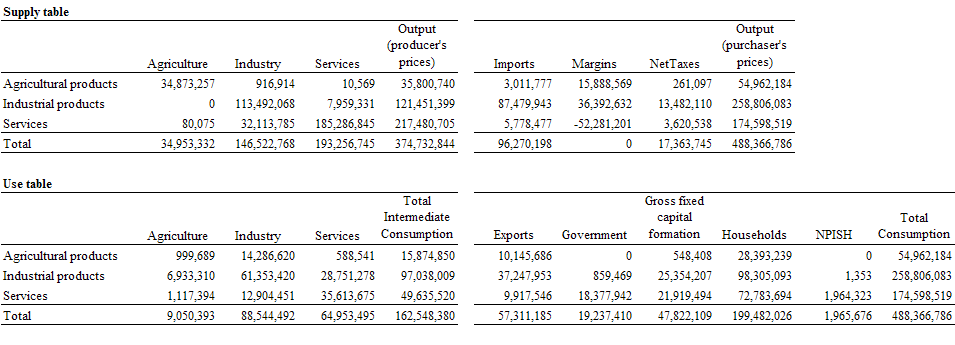
\includegraphics[width=6in]{supuse}
\centering
\textbf{\textit{Element about here.}}
\end{center}
\label{supuse}
\end{table}

The use portion in table \ref{supuse} also shows that the $C$ in equation \ref{eq1} is split, in practice, between intermediate consumption, performed by industries, and final consumption expenditures, done primarily by households (along with exports, gross fixed capital formation, non-profit organizations serving households, and the government).  

From this configuration of the SNA, calculation of gross domestic product is straight forward. The value added by any individual industry to the economy is what is left from substracting the value of intermediate inputs from total output of that industry. The sum of the individual value added components accross all industries (plus net government participation in the economy in the form of taxes less subsidies on products) yields GDP.

In order to exploit the mathematical and analytical benefits of the Leontief approach, the supply and use tables of the Guatemalan economy had to be converted into input-output tables. While the SNA manual itself \citep{sna2009} suggests an approach for the construction of such tables, it encourages what is known as an \mbox{industry-by-industry} configuration in order to build a square matrix that represents purchases of economic activities made to other activities and themselves, as initially proposed by \citet{leontief_1947}. However, since the number of commodities in supply and use tables does not match the number of industries that produce them\footnote{This means that every industry can produce more than one product and products can simultaneously be produced by two or more industries.}, the \mbox{industry-by-industry} approach loses valuable disaggregated information on primary and secondary production. At the same time, it requires the acceptance of unnecessary assumptions regarding reallocation of secondary production. For that reason, this study uses a \mbox{commodity-by-industry} approach that allows for calculations that retain the benefits of commodity disaggregation\footnote{I later sketch the \mbox{commodity-by-industry} approach briefly, but the interested reader can turn to chapter 5 of \citet{miller2009} for a detailed explanation.}. 

The diagram from figure \ref{fig02} is the blueprint of the commodity-by-industry system used to organize the data from the supply and use tables for analysis. $\underset{(c\times i)}{\mathbf{U}}= [u_{ij}]$ in the diagram is the \textit{Use} matrix, which has dimensions commodities-by-industries and where each individual element of it $u_{ij}$ is the value of purchases of commodity $i$ by industry $j$. It is also known as the \textit{absorption} or \textit{input} matrix. $\underset{(i\times c)}{\mathbf{V}}= [v_{ij}]$ is the \textit{Make} matrix which shows how industries make commodities. Each element of it $v_{ij}$ represents the value of the output of commodity $j$ that is produced by industry $i$ and is also called the \textit{output} matrix. The vector resulting from the row sum of $\mathbf{V}$ is the total industry output $(\mathbf{v})$. Similarly, total commodity output $(\mathbf{q'})$ can be calculated as the column sum of $\mathbf{V}$.  The commodity final demand vector $(\mathbf{e})$, with elements $e_i$ and the row vector of value added by industries $(\mathbf{v'})$ are also represented.


\begin{figure}[!hbtp]
\begin{center}
%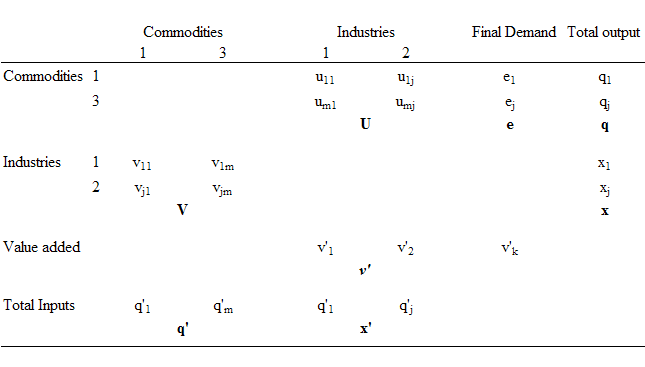
\includegraphics[width=5in]{fig02}
\centering
\textbf{\textit{Element about here.}}
\end{center}
\caption{Commodity-Industry complete set diagram.}
\label{fig02}
\end{figure}


\subsubsection{From purchasers prices to producer prices: trade and transportation margins}

The first step in the construction of a set of consolidated \mbox{commodity-by-industry} \mbox{input-output} accounts, both supply and use tables have to express transactions in the same terms (or set of prices). The supply table is in producers prices (or prices at the factory door) and further expenses in trade, transportation, and utilities are used to bring the commodities to the final point of purchase where it is sold to other economic sectors as inputs in their production or to households, the government, etc. as final demand at purchasers prices. Each individual transaction in the use table reflects those margins. Since the overall value corresponding to each type of margin is known from our supply table in the complete version of figure \ref{fig01} for each commodity at the total output level, the assumption is made that, for every commodity, the same proportion holds for each individual purchase of it.

From there a simple reconfiguration of the data is made. We factor each margin out (substract from each row) of the use table and we add them together into a single row vector.  Then we take that vector and re-add it to the use table, only we add to the row that represents the ``commodity'' or service that is the margin. In this case, we factor out four such vectors. One for transportation services, one for trade services, one for electricity, and one for water service. In essence, what is done is basically transforming the margins into service inputs to each industry, removing flows through the trade, transportation, and utility sectors, since this would depict an economy where industries and final customers would make most of their purchases from and sales to the trade, transportation, and utilities industries alone. We name the resulting matrix $\mathbf{\tilde{U}}$ as a previous step in the construction of $\mathbf{U}$ in figure \ref{fig02}.

All final demand components also pay those margins when they purchase commodities, so the same procedure is applied to the final demand vector. All purchases of commodities are reduced by the fraction that stands for the margins and those fractions are re-added as purchases of the services those margins represent. We name the resulting vector $\mathbf{\tilde{e}}$ as a previous step in the construction of $\mathbf{e}$. In what follows, a tilde (\~{}) will be used to denote a version of any element in figure \ref{fig02} which still contains taxes and competitive imports.

\subsubsection{From purchasers prices to producer prices: competitive imports and taxes on products}
\label{imports}

The matrix $\mathbf{\tilde{U}}$ constructed in the previous step, additional to direct allocations of commodities, still contains net taxes\footnote{Taxes less subsidies on products.}, and imports. The problem is that we are interested in national interindustry transactions for which it is known that the technical coefficients apply. Otherwise, impacts in modifications to final demand would be felt by foreign producers with local technology, which does not make sense. Similarly, with the government and product taxes.  There is a need to ``scrub'' those elements out (or remove them). The assumption is made that there are matrices that are known which can be added to the wanted matrix $\mathbf{U}$ that contain those extra elements in order to bring it to purchaser prices. Those matrices are termed $\mathbf{U^m}$ for a matrix of imports and $\mathbf{U^t}$ for a matrix of taxes so that

\begin{equation}
\mathbf{\tilde{U}} =  \mathbf{U} + \mathbf{U^m} + \mathbf{U^t},
\label{eq4.02}
\end{equation}

The problem is that in this case the last two matrices are not known and have to be estimated. From the supply and use tables the vector of total imports by commodity $(\mathbf{m})$ and the vector of total taxes by commodity $(\mathbf{t})$ are known. The simplifying assumption is made that for each industry the fraction of a given input supplied by imports is the same and that that fraction also applies to consumer and government expenditures, then for each industry that fraction is given by $r_i$ so that $m_i = r_i x_i$, and it can be estimated by

\begin{equation}
r_i = \frac{m_i}{u_i + e_i}.
\label{eq4.03}
\end{equation}

This yields the vector of commodity import fractions $(\mathbf{r})$ that can be used to estimate the interindustry imports matrix and the final demand imports vector by

\begin{equation}
\mathbf{\bar{U}^m} = \mathbf{\hat{r}\tilde{U}}.
\label{eq4.04}
\end{equation}

Taxes are dealt with in the same way, assuming that the fraction of a given input that represents taxes is the same for each industry and that that fraction also applies to final demand consumption. Then, for each industry that fraction is given by $s_i$ so that $t_i = s_i x_i$, and it can be estimated by

\begin{equation}
s_i = \frac{t_i}{u_i + e_i}.
\label{eq4.05}
\end{equation}

This yields the vector of commodity tax fractions $(\mathbf{s})$ that can be used to estimate the interindustry taxes matrix by

\begin{equation}
\mathbf{\bar{U}^t} = \mathbf{\hat{s}\tilde{U}},
\label{eq4.06}
\end{equation}

Rearranging equation (\ref{eq4.02}) and using equations (\ref{eq4.04}) and (\ref{eq4.06}) the working \textit{Use} matrix is calculated by

\begin{equation}
\mathbf{U} = \mathbf{\tilde{U}} - \mathbf{\hat{r}\tilde{U}} - \mathbf{\hat{s}\tilde{U}}.
\label{eq4.07}
\end{equation}

Finally, the same procedure is used to scrub out imports and taxes from the final demand vector $(\mathbf{\tilde{e}})$, assuming that it is the sum of the wanted vector $(\mathbf{e})$, an imports final demand vector $(\mathbf{e^m})$, and a tax final demand vector $(\mathbf{e^t})$. Using the fractions calculated from (\ref{eq4.03}) and (\ref{eq4.05}) the final demand vector is calculated as:

\begin{equation}
\mathbf{e} = \mathbf{\tilde{e}} - \mathbf{\hat{r}\tilde{e}} - \mathbf{\hat{s}\tilde{e}}.
\label{eq4.08}
\end{equation}
 
\subsubsection{The final commodity-by-industry input-output tables}

Before building the input-output model, minor adjustments were conducted on the original supply and use tables. The number of industries was reduced, first to eliminate sectors that apparently were considered by the SNA developers when designing the Guatemalan system, but later were not compiled due to impossibility of disassociating its components from umbrella industries, leaving zeros, both in the supply and in the use table. Additionally, the system separates production in market, non-market, and final own use output using a subset of the same industries (repeating them) in the three sections. Since this distinction is not relevant for this study, the columns in the non-market and final own use sections were added to their counterparts in the market section, bringing the system down from 143 industries to 122. Following convention and as suggested by an important study \citep{nrc_2006}, noncompetitive imports\footnote{Noncompetive imports are those products that are not produced locally so whatever amount of them that is used by the economy is imported in its entirety.}, which are not dealt with in section \ref{imports}, were treated as local production, assigning them to a new industry that has no inputs. They are properly discounted in their entirety, adjusting them negatively in final demand. Some of those imports are of importance for this study, like gasolene and liquefied petroleum gases. Thus, the final system has a total of 123 sectors or industries. Consequently, commodities that showed zeros in ouput, input, and final demand were extracted from the study, leaving a total of 219 commodities from the original 226 considered in the Guatemalan SNA. Aggregated versions of the \textit{Use} matrix ($\mathbf{U}$) and the \textit{Make} matrix ($\mathbf{V}$) are presented in tables \ref{tab4.01} and \ref{tab4.02}, respectively. Final demands are presented later, in section \ref{findem}, where particularities of construction of final demand vectors for urban and rural households are explained.


\begin{table}
  \caption{Aggregated \textit{Use} matrix ($\mathbf{U}$) of Guatemala (2006, in thousands of GTQ)}
%	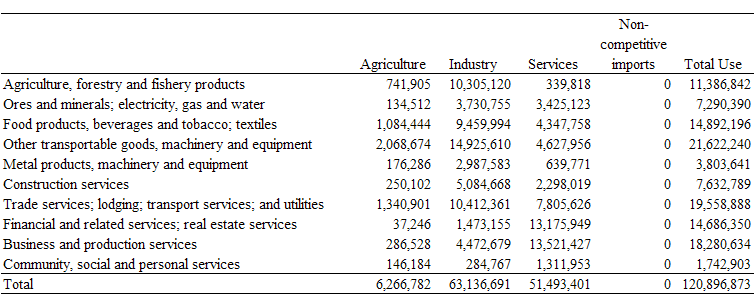
\includegraphics[width=5in]{use}
\centering
\textbf{\textit{Element about here.}}
	\label{tab4.01}
\end{table}


\begin{table}
  \caption{Aggregated \textit{Make} matrix ($\mathbf{V}$) of Guatemala (2006, in thousands of GTQ)}
%  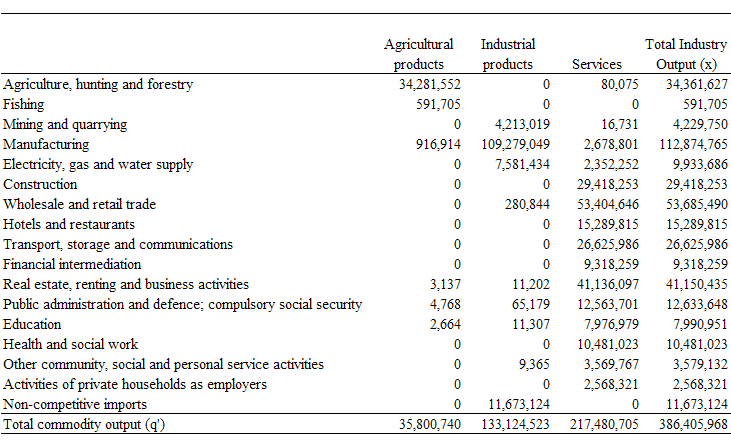
\includegraphics[width=5in]{make}
\centering
\textbf{\textit{Element about here.}}
	\label{tab4.02}
\end{table}



\subsection{Environmental Accounting and Energy}
\label{seea}

The SEEA is a framework which expands the accounting structure of the System of National Accounts (SNA) and addresses known shortcomings found in it, regarding the treatment of the environment \citep{lange_2007}. Those shortcomings include the SNA failure to consider natural resource depletion as consumption of (natural) capital stocks \citep{repetto_2007}; thus, treating what is essentially a form of depreciation, as income or wealth generation. The set of accounts that comprise the SEEA provides a common structure for registering economic and environmental information that allows for a standard assessment of the contribution of the environment to the economy and of the impact of the economy on the environment \citep{seea_2003}. More specifically for this study, it provides a set of accounts related to the physical use of different energy commodities, as well as to greenhouse gas emissions produced by their consumption.

Whereas the implementation of the SEEA has been widespread in the developed world, developing countries have shown a slower progress in its adoption, despite that for those nations ``natural capital usually forms a relatively larger share of the overall capital portfolio, (\ldots) and (\ldots) resource depletion has imperiled livelihoods and economic development''  \citep{repetto_2007}. Following this, formal research based on information compiled or generated by said system has been conducted much more frequently on data provided by statistical offices from developed nations. For example, combining the data on production and consumption generated by SNA and estimates on natural resource use from SEEA, much work has been done in the areas of input-output modeling and applied general equilibrium models (for example, \citealp{serrano_2010}; \citealp{wissema_2007}). The Guatemalan SEEA added to exercises in environmental accounting conducted in transition economies and development countries such as India, Indonesia, China, the Philippines, Thailand, Mexico, Brazil, Colombia, Chile, Botswana, Namibia, Cote d'Ivoire, and the Dominican Republic, among others. 

The results yielded by the particular subset of SEEA accounts related to energy reveal a strong dependence of the Guatemalan households on fuelwood, a phenomenon with little attention within the literature of input-output analysis, presumably given the different set of priorities faced by industrialized countries. Figure \ref{fig03} shows consumption for all groups of economic activity (sectors) in Guatemala of 11 energy commodities, as inputs in production (intermediate consumption) as well as for final demand of households and the government, expressed in terajoules (\tera\joule) for the year 2006.  Of the 483,947.3 \tera\joule{} of energy consumed in the country, 39\% corresponds to household use of fuelwood (188,501.2 \tera\joule), which is, by itself, larger than any single industrial use of each of the fuel commodities considered. Fuelwood is used primarily for cooking by households.

\begin{figure}[!hbtp]
	\centering
%		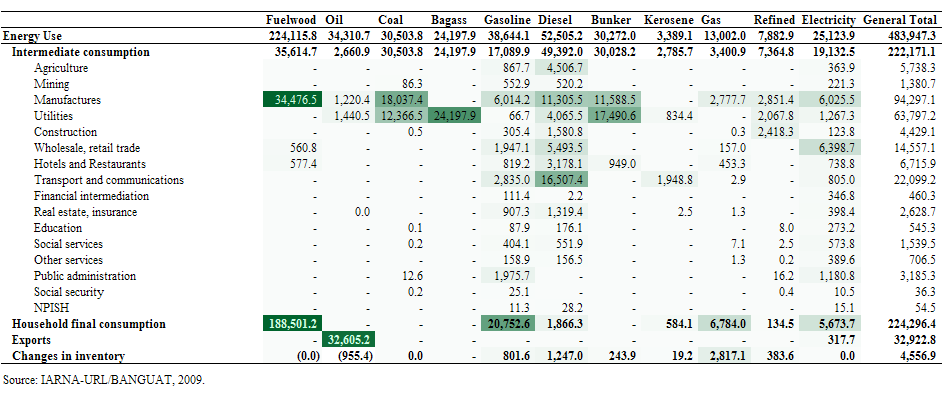
\includegraphics[width=6in]{ciee}
\textbf{\textit{Element about here.}}
	\caption{Guatemala: Energy use (in \tera\joule)}
	\label{fig03}
\end{figure}

Using data from the energy accounts on the individual consumption of energy (in \tera\joule), for each sector and for 11 energy commodities, as well as domestic output information from the \textit{Make} matrix ($\mathbf{V}$), it was possible to construct a ($11\times123$) matrix of energy impact coefficients, denoted $\mathbf{M_p}$. This matrix states how much of each energy commodity is expected to be used by every monetary unit (GTQ) of output for each industry. 

The energy use matrix is created in a ($123\times11$) industry-by-energy commodity arrangement (in \tera\joule) and it is called $\mathbf{E}$.  If that is true, then dividing every energy use of industry $j$ by the output of that industry ($\mathbf{x}$ from figure \ref{fig02}) will yield the matrix of energy impact coefficients from equation (\ref{eq31.04}).

\begin{equation}
\mathbf{M_p} = \mathbf{E\hat{x}^{-1}}
\label{eq31.04}
\end{equation}


A similar ($11\times1$) vector, denoted $\mathbf{M_h}$ was created in order to account for energy use per monetary unit of household final demand. 

\subsection{\mbox{Encovi 2006}: Splitting the household consumption vector into urban and rural}
\label{findem}

The final demand vector is constructed by summing household consumption with the consumption of nonprofits, the government, net exports, and elements of gross capital formation. All these elements account for all output that is not consumed as intermediate inputs by other enterprises. Table \ref{tab4.03} shows these components for the Guatemalan case. The main interest of this study is the analysis of the impacts of demographic change (urban and rural) on energy use so the vector of final demand was manipulated in order to establish that change exogenously. The idea was to show that urban final demand is expected to grow quicker than rural demand and thus the ``product mix'' of total households had to change in order to reflect the preferences of an urban component larger than its rural counterpart. For that, the household final demand vector given by the SNA had to be split into its urban and rural components.

\begin{table}
  \caption{Domestic final demand ($\mathbf{e}$) of Guatemala (2006, in thousands of GTQ)}
%	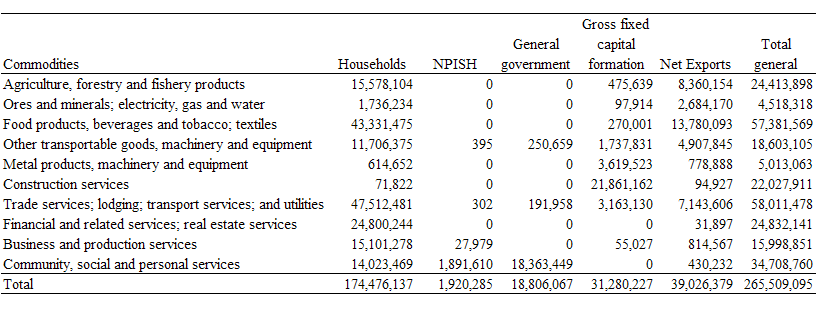
\includegraphics[width=5in]{findemand}
\centering
\textbf{\textit{Element about here.}}
	\label{tab4.03}
\end{table}


In order to differentiate between households coming from the urban and rural groups, consumption was sorted accordingly using data from ENCOVI 2006. The assumption that households within each group are homogeneous was made during this process, following the approach of \citet{kronenberg09}.  The total consumption expenditure of a household was differentiated by consumption purposes. For each consumption purpose $m$, a consumption coefficient $\gamma^m_g$ was defined as the expenditure share of consumption purpose $m$ in total consumption. In that manner, the expenditure of the average household from group $g$ on consumption purpose $m$ was written as:

\begin{equation}
c^m_g = \gamma^m_g c_g
\label{eq32.01}
\end{equation}

where $c_g$ denotes the total consumption expenditure of a household in group $g$ and $c^m_g$ refers to the expenditure on consumption purpose $m$. Since homogeneity within each group was assumed, the total consumption expenditure of group $g$ on consumption purpose $m$ was calculated by multiplying $c^m_g$ with the number of households $H_g$:

\begin{equation}
C^m_g = H_g c^m_g 
\label{eq32.02}
\end{equation}

Consequently the total expenditure for a consumption purpose $m$ was determined by summing over groups in the following manner:

\begin{equation}
C^m = \sum_{g=1}^{\tilde{g}} \\ C^m_g
\label{eq32.03}
\end{equation}

where $\tilde{g}$ denotes the number of groups, equal to two: urban and rural. A combination of equations \eqref{eq32.01} to \eqref{eq32.03} were used to build an expression for consumption expenditure by consumption purpose:

\begin{equation}
C^m = \sum_{g=1}^{\tilde{g}} H_g \gamma^m_g c_g
\label{eq32.04}
\end{equation} 

Using correspondence tables, all consumption purposes are reallocated to the central product classification (CPC) from the COICOP classification in order to obtain the total consumptions of urban and rural households on the same terms as the commodities in the \textit{Use} and \textit{Make} matrices. From this, coefficients of urban and rural consumption were calculated from total consumption for each commodity. These coefficients, rather then the actual consumption totals, were used to split the SNA household vector in two. The reason why this was done is because the vector in national accounts has gone through a process of harmonization with the system, where subreporting has been corrected by the compilers, taking into account information from enterprise sales surveys and other adjustment methods.

The number of commodities in CPC terms taken into account in the SNA is larger than that accounted for by the ENCOVI household survey\footnote{The number of products in ENCOVI is considerably larger than that of commodities in SNA, but several are grouped into single CPC categories when reallocating from COICOP, such as processed food products.}, so for 15 of the 219 commodities the assumption had to be made that their urban and rural household consumption coefficients were similar to other products in the same classification bracket, either by copying the coefficients of a single other product in their bracket or by calculating a weighted average of two or more other commodities in their bracket. The final result is a differentiated product mix that reflects the different preferences of urban and rural households. Table \ref{tab4.04} shows an aggregated version of the calculated vectors.


\begin{table}
 \caption{Urban and rural household domestic final demand ($\mathbf{e}$) of Guatemala (2006, in thousands of GTQ)}
%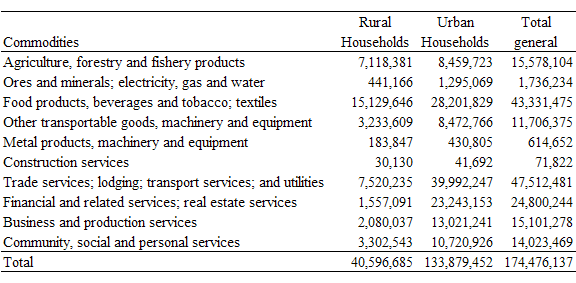
\includegraphics[width=5in]{urbrur}
\centering
\textbf{\textit{Element about here.}}
	\label{tab4.04}
\end{table}


\section{Input-Output Analysis}

After preparation of the data, an imput-output model was created. We started with the original model by \citet{leontief_1947} which is based on an industry-by-industry approach, where transactions are made between economic sectors. Modifications were then conducted in order to account for the commodity-by-industry configuration of the data. In the original model the matrix $\mathbf{Z}=[z_{ij}]$ stands for purchases of industry $i$ output by industry $j$. There is also a vector of total industry outputs, $\mathbf{x}=[x_j]$ and there are also industry $j$'s sales to final demand ($f_j$), which put together express that


\begin{equation}
x_j=z_{j1}+\cdots+z_{jn}+f_j,
\label{eq5.01}
\end{equation} 

\noindent which expressed in matrix form, reads

\begin{equation}
\mathbf{x = Zi + f}.
\label{eq5.02}
\end{equation}

Consequently, direct input (technical) coefficients can be defined as $\mathbf{A}=[a_{ij} = \frac{z_ij}{x_j}]$ and expressed in matrix form as

\begin{equation}
\mathbf{A = Z\hat{x}^{-1}}.
\label{eq5.03}
\end{equation}

In the commodity-by-industry approach it is necessary to find parallels for these elements. The obvious first step is to replace $\mathbf{Z}$ with the \textit{Use} matrix $\underset{(c\times i)}{\mathbf{U}}= [u_{ij}]$ that we obtained in equation \ref{eq4.07}. Additionally, similar to the direct input coefficients $\mathbf{A}$, we obtain an homologous measure from $u_{ij}/x_j$, which in matrix terms reads

\begin{equation}
\mathbf{B = U\hat{x}^{-1}}
\label{eq5.04}
\end{equation}

\noindent and represents the value of inputs of each commodity per monetary unit's worth of industry $j$'s output and has commodities-by-industries dimensions. We then recall $\mathbf{V}$ from figure \ref{fig02} and table \ref{tab4.02} and use it to find total industry output

\begin{equation}
\mathbf{x = Vi}
\label{eq5.05}
\end{equation}

\noindent and total commodity output by

\begin{equation}
\mathbf{q =(V')i}
\label{eq5.06}
\end{equation}

\noindent as well as from figure \ref{fig02}

\begin{equation}
\mathbf{q =Ui+e}
\label{eq5.07}
\end{equation}

As a paralell to the usage of (\ref{eq5.02}) and  (\ref{eq5.03}), here (\ref{eq5.07}) and (\ref{eq5.04}) are used. Substituting the former into the latter we obtain

\begin{equation}
\mathbf{q =Bx+e},
\label{eq5.08}
\end{equation}

\noindent which is our parallel to the ordinary input-output model. However, since ($\mathbf{q}$) on the left-hand side has commodity output and ($\mathbf{x}$) on the right-hand side has industry output a total requirements matrix cannot be generated. In order to solve this problem an alteration has to be made, transforming either industry outputs to commodity outputs or transforming commodity outputs and final demand into industry terms.

If we define $d_{ij}= \frac{v_{ij}}{q_j}$ in a manner that it denotes the fraction of total commodity $j$ output that was produced by industry $i$ we obtain 

\begin{equation}
\mathbf{D=V\hat{q}^{-1}},
\label{eq5.09}
\end{equation}

\noindent which has industries by commodities dimensions and is called the \textit{market shares matrix}. By definition, each column sum is unity.

With this linear transformation we can now use it in conjunction with (\ref{eq5.05}) to establish that

\begin{equation*}
\mathbf{D=V\hat{q}^{-1}} \Rightarrow \mathbf{D\hat{q}= V} \Rightarrow \mathbf{D\hat{q}i} = \mathbf{Vi}
\label{eqtottrf}
\end{equation*}
 
\noindent so from (\ref{eq5.05})

\begin{equation}
\mathbf{Dq=x},
\label{eq5.10}
\end{equation}

The relationships made evident here reveal the unity of the system if we understand from (\ref{eq5.10}) that $\mathbf{x-Dq=0}$, and from (\ref{eq5.08}) that $\mathbf{-Bx+q=e}$. These matrix equations in $\mathbf{x}$ and $\mathbf{q}$ represent the following partitioned matrix system:

\begin{equation*}
\begin{bmatrix}
\mathbf{I} & \mathbf{-D} \\
\mathbf{-B} & \mathbf{I} 
\end{bmatrix} 
\begin{bmatrix}
\mathbf{x} \\
\mathbf{q}
\end{bmatrix} 
=
\begin{bmatrix}
\mathbf{0} \\
\mathbf{e}
\end{bmatrix}
\label{partmat}
\end{equation*}

So in order to solve the issue of having both $\mathbf{x}$ and $\mathbf{q}$ in (\ref{eq5.08}) it is possible to premultiply both sides there by $\mathbf{D}$, and since $\mathbf{Dq=x}$ we have that 
 
\begin{equation*}
\mathbf{x = DBx + De}
\label{another}
\end{equation*}

\noindent and finally the transformation is made to 

\begin{equation}
\mathbf{x = [(I-DB)^{-1} D] e},
\label{eq5.11}
\end{equation}

\noindent which is the final industry-by-commodity total requirement matrix, parallel to $\mathbf{x=(I-A)^{-1} f= Lf}$ from the original model.

One last step is necessary to complete the model, however. In this study, the primary interest is not on the final output modeled taking demographic change into account, but on the future energy use, and specifically, fuelwood use. In section \ref{seea} we created a matrix of impact coefficients by energy commodity for every industry, which we termed $\mathbf{M_p}$. Premultiplying $\mathbf{x}$ by it yields a $(12\times1)$ vector containing the total energy use of each of the 12 commodities that are explored, including fuelwood. This is done using (\ref{eq5.11}) to obtain

\begin{equation}
\mathbf{E_p = M_p [(I-DB)^{-1} D] e},
\label{eq5.11}
\end{equation}

\noindent which is our working model. This model yields the energy use of industries and, adding it to its counterpart calculated directly from $\mathbf{M_h}$ and $\mathbf{e}$, we obtain the total energy use for the entire system.


\section{Modelling demographic change}

The model derived in the previous section is the base case for Guatemala for the year 2006. It is a representation of the relationships between economic sectors and final demand. If we make the assumption that those relationships are structural and are not going to change dramatically in the near future it is possible to ask what would happen if the exogenous final demand sees changes in its composition due to demographic conditions such as population growth or migration.

It is known from the population projections of Guatemala (Table \ref{tab6.01}) that in the 15 years evaluated by this study, urban areas will experience a more rapid population growth than their rural counterparts, presumably because the natural growth rate in them is complemented with high rates of rural-urban migration. For this reason, we use the differentiated growth rates to alter the urban and rural household final demand vectors derived in section \ref{findem} separately, which in turn alters the commodity use shares of their total.

By dividing the entire demand vectors by the total population in the base year we obtain a consumption vector per capita. If we then multiply that by the population projection for the desired year, we obtain the hypothetical household demand vector for that year.  Such a calculation was conducted in two ways. In the first case, which will be called uncorrected, the joint total household vector was incremented according to the national population growth for every year analyzed, without differentiating between urban and rural. This served as a control case, which is the equivalent of only incrementing the entire system by the growth rate, yielding an energy use increment of the same magnitude.

For the second case, which will be referred to as the corrected one, the differentiated vectors of final demand derived in section \ref{findem} were used in order to change the urban and rural household demand vectors in a differentiated manner, adjusting the first according to the urban growth rate and the second taking into account the rural growth rate. These vectors are added back into a total household demand, but given that the use mix, not only of energy commodities, but of all products, is different between the two groups, shifts in the overall commodity expenditures shares were expected, with different results in the economy, as indirect impacts are carried out by backward linkages between economic activities in a differentiated manner.

Rather than feeding a single vector $\underset{(219\times1)}{\mathbf{e}}$ to the model above, two matrixes with dimensions ($219\times15$) representing commodities-by-years were created for each of the cases explained above, in order to have results for every year of the analysis. Since the model yielded originally one single ($12\times1$) vector of energy commodity use by the total economy, by changing the final demand vector to a series of them representing the various years, the result of the model is a ($12\times15$) vector of 12 energy commodities uses for each of the 15 years analyzed. Finally, a conversion factor given by the Guatemalan SEEA is used in order to translate terajoules of fuelwood into cubic metres of forest resource.


\begin{table}
  \caption{Guatemalan population projections (2006-2020) (no. of inhabitants)}
%  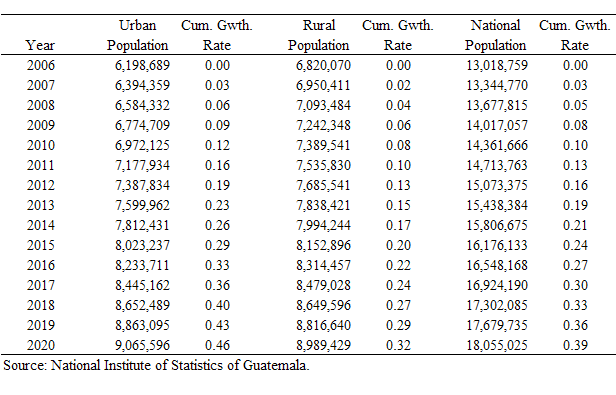
\includegraphics[width=5in]{population}
\centering
\textbf{\textit{Element about here.}}
	\label{tab6.01}
\end{table}


\section{Findings and discussion}

%\subsection{Fuelwood}

One of the main interests of this paper was determining whether the changes in the urban and rural structure of the population due to demographic phenomena, such as growth and migration, had a distinct impact on the use of fuelwood, not only by the Guatemalan families, but also by the producing sectors, given a different consumption level. It was hypothesized that this could ease the pressure on forests.

Partial support for these ideas was found in the resulting calculations. For example, when correcting for urban and rural growth rates, household consumption of fuelwood at the end of the analysis period (2020) is 1.7\% lower than what it would be if an estimation was conducted without correcting for the difference in growth rates, with respect to the base year (2006). That is an equivalent of $408,563.5\metre\cubic{}$ of wood that translate into less pressure on forests, as shown in table \ref{tab7.01}. However, since there are still high growth rates in both areas, regardless of their difference it is not possible to expect a considerable drop in fuelwood use at the national level. On the contrary, a total of $307,082.1\tera\joule{}$ of wood energy, or $33,615,990.5\metre\cubic{}$ of wood can still be expected to be needed for those purposes in the year 2020, as a consequence of higher demand brough upon by demographic change; a result that holds if preferences or production technologies do not change radically. Differences from the uncorrected case can be seen in figure \ref{fig04} for all energy commodities. 

\begin{figure}[]
\begin{center}
%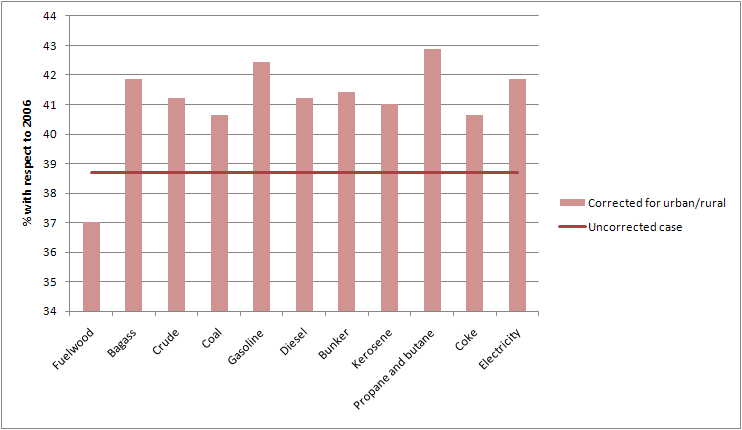
\includegraphics[width=5in]{differences}
\centering
\textbf{\textit{Element about here.}}
\end{center}
\caption{Differences in energy use, corrected and uncorrected case for the year 2020, with respect to the Base year (2006)}
\label{fig04}
\end{figure}

It is noteworthy that here the linkages in the economy play an important role. When looking at the corrected household final energy demand ($\mathbf{E_p}$) and the corrected industry energy demand ($\mathbf{E_p}$) separately, an interesting phenomenon can be observed. For the first one, the difference between the uncorrected and the corrected case is larger than in the global case explained before (of 2.5\% with respect to the base year 2006). Nevertheless, since the urban share of consumption grows faster, changing the total household commodity use shares, it induces a bigger demand of other commodities that use fuelwood as inputs in their production. That means that for the corrected industry energy demand, fuelwood use is expected to be 2.8\% higher than that of the uncorrected case, partially offseting the household result. In spite of that, the offset is not significant, because over 80\% of the fuelwood is consumed by households in the base year.

\begin{table}
	\caption{Estimated fuelwood use (2006-2020) ($\metre\cubic{}$)}
\begin{center}
% 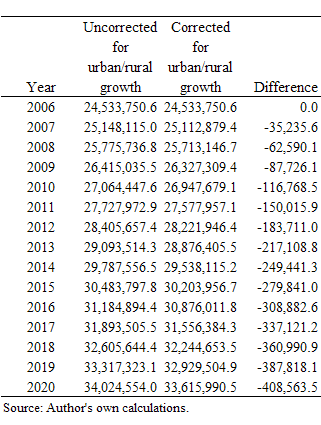
\includegraphics[width=5in]{fuelwood}
\centering
\textbf{\textit{Element about here.}}
\end{center}
	\label{tab7.01}
\end{table}

This issue is much more significant for kerosene. In the corrected version of the houselhold energy consumption vector, 5.6\% less of that commodity is expected to be used than in the uncorrected version, with respect to the base year 2006. Notwithstanding, by modifying the commodity consumption shares in final demand due to demographic reasons, a higher consumption of commodities that use kerosene as an input is induced through secondary impacts in the economy, boosting its industry use to 4\% higher than in the uncorrected case with respect to 2006, completely offsetting the negative effect of households and leaving the total energy use 2.3\% higher than expected for a total of $4,751.8\tera\joule{}$.

The opposite is true for propane or butane gases (cooking gases). As expected, the urbanization process induces an increase in the use of such commodities for use in the kitchen, sometimes replacing fuelwood entirely, and sometimes complementing its use. Aditionally, there is a marked incresase in the use of those gases by industries that use them as inputs in their production. For that reason, in the corrected case the use of propane or butane is 4.2\% higher than in the uncorrected version, with respect to the base year. The same is true for electricity ($3.2\%$), gasoline (3.7\%), and diesel (2.5\%) which were expected to be higher as the urban share became larger in comparison to the uncorrected case.

It is interesting to see that bagass is also different than expected in an important manner (3.2\%). In Guatemala, bagass is a waste of sugar cane agriculture, which is used as fuel in order to heat water. In that process, water is turned into steam and it is used to move turbines for electricity production. Given that, a larger share of urban homes induces a larger use of electricity, both directly as indirectly, bagass demand is incremented accordingly as an input in that industry.

Finally, table \ref{tab7.02} shows the total energy demands for all energy commodities during even years of the analysis period. Fuelwood will continue to be the main source of energy for the country in absolute terms (in \tera\joule{}) with a share of $49.4\%$; followed by diesel (11.6\%), which powers most of the transportation of goods, services, and passengers; gasoline, which is used mainly in household vehicles, but also in commercial vehicles (8.7\%); coal, used exclusively in electricity production (6.9\%); bunker, used as fuel for industrial boilers (6.8\%); electricity (5.6\%); bagass (5.5\%); propane and butane gases, used for cooking by households (2.3\%); and the remaining commodities (3.2\%). 

\begin{table}
	\caption{Total Guatemalan energy use by type of energy commodity (2006-2020; selected years) (in $\tera\joule{}$)}
%  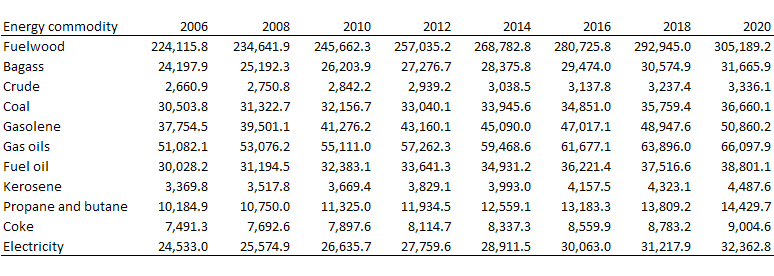
\includegraphics[width=5in]{totalenergy}
\centering
\textbf{\textit{Element about here.}}
	\label{tab7.02}
\end{table}

\section{Conclusion}

Although modest changes in the structure of energy commodity shares of Guatemala are expected\footnote{About 1\% that is taken away from the share of fuelwood use and redistributed among the other energy commodities during the 15 years of the analysis.} under this input-output analysis, it is evident that demographic change alone, in terms of migration and growth, cannot be presumed to induce large shifts in consumption during a period of 15 years. The fact that fuelwood will continue to represent such a large share of the total energy needs of the country should be of concern for policy makers, given that the pressure on forests will only aggravate as populations continue to grow. It is important to acknowledge that there is a natural limit to how much fuelwood can be extracted from the forest until damages become irreversible in the short run. 



%\theendnotes

%\appendix

%\section{The First Appendix}

%The appendix fragment is used only once. Subsequent appendices can be created
%using the Section Section/Body Tag.

\newpage
\bibliography{LPR_Vargas}
%\nocite{*}

\end{document}


